

\tikzset{every picture/.style={line width=0.75pt}} %set default line width to 0.75pt        

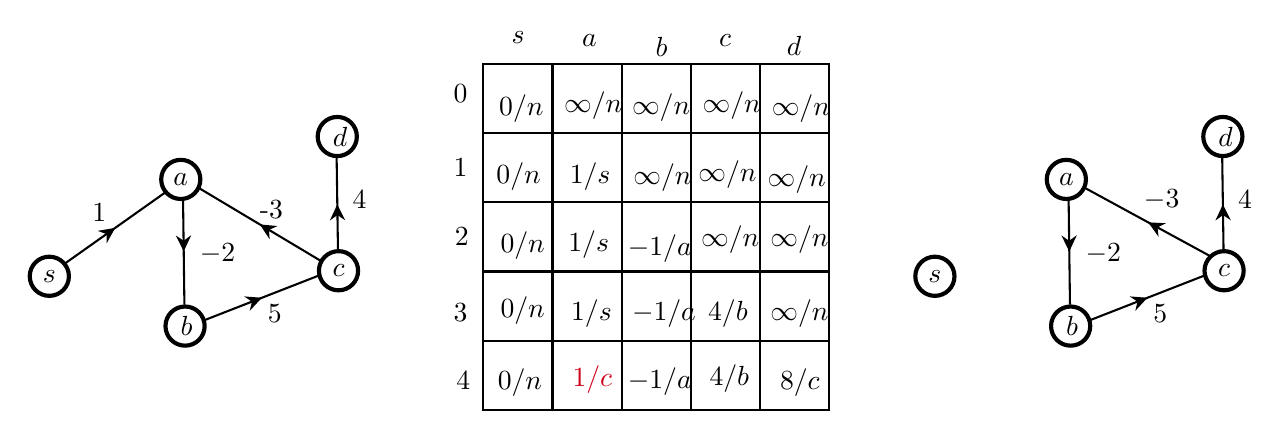
\begin{tikzpicture}[x=0.5pt,y=0.5pt,yscale=-1,xscale=1]
%uncomment if require: \path (0,334); %set diagram left start at 0, and has height of 334

%Shape: Grid [id:dp11668880045661734] 
\draw  [draw opacity=0] (352,45) -- (602,45) -- (602,295) -- (352,295) -- cycle ; \draw   (402,45) -- (402,295)(452,45) -- (452,295)(502,45) -- (502,295)(552,45) -- (552,295) ; \draw   (352,95) -- (602,95)(352,145) -- (602,145)(352,195) -- (602,195)(352,245) -- (602,245) ; \draw   (352,45) -- (602,45) -- (602,295) -- (352,295) -- cycle ;
%Straight Lines [id:da34498379019209924] 
\draw [color={rgb, 255:red, 0; green, 0; blue, 0 }  ,draw opacity=1 ][line width=0.75]    (50,189) -- (122,138) ;
\draw [shift={(86,163.5)}, rotate = 504.69] [fill={rgb, 255:red, 0; green, 0; blue, 0 }  ,fill opacity=1 ][line width=0.08]  [draw opacity=0] (11.61,-5.58) -- (0,0) -- (11.61,5.58) -- (7.71,0) -- cycle    ;
%Straight Lines [id:da15240395104529547] 
\draw [color={rgb, 255:red, 0; green, 0; blue, 0 }  ,draw opacity=1 ][line width=0.75]    (147,135) -- (234,187) ;
\draw [shift={(190.5,161)}, rotate = 30.87] [fill={rgb, 255:red, 0; green, 0; blue, 0 }  ,fill opacity=1 ][line width=0.08]  [draw opacity=0] (11.61,-5.58) -- (0,0) -- (11.61,5.58) -- (7.71,0) -- cycle    ;
%Straight Lines [id:da35482909520855144] 
\draw [color={rgb, 255:red, 0; green, 0; blue, 0 }  ,draw opacity=1 ][line width=0.75]    (233,198) -- (151,230) ;
\draw [shift={(192,214)}, rotate = 158.68] [fill={rgb, 255:red, 0; green, 0; blue, 0 }  ,fill opacity=1 ][line width=0.08]  [draw opacity=0] (11.61,-5.58) -- (0,0) -- (11.61,5.58) -- (7.71,0) -- cycle    ;
%Straight Lines [id:da9934926023449607] 
\draw [color={rgb, 255:red, 0; green, 0; blue, 0 }  ,draw opacity=1 ][line width=0.75]    (135,142) -- (136,219) ;
\draw [shift={(135.5,180.5)}, rotate = 269.26] [fill={rgb, 255:red, 0; green, 0; blue, 0 }  ,fill opacity=1 ][line width=0.08]  [draw opacity=0] (11.61,-5.58) -- (0,0) -- (11.61,5.58) -- (7.71,0) -- cycle    ;
%Straight Lines [id:da7563500509285274] 
\draw [color={rgb, 255:red, 0; green, 0; blue, 0 }  ,draw opacity=1 ][line width=0.75]    (246,112) -- (247,181) ;
\draw [shift={(246.5,146.5)}, rotate = 89.17] [fill={rgb, 255:red, 0; green, 0; blue, 0 }  ,fill opacity=1 ][line width=0.08]  [draw opacity=0] (11.61,-5.58) -- (0,0) -- (11.61,5.58) -- (7.71,0) -- cycle    ;
%Straight Lines [id:da1926158580753592] 
\draw [color={rgb, 255:red, 0; green, 0; blue, 0 }  ,draw opacity=1 ][line width=0.75]    (787.5,135) -- (877.5,184) ;
\draw [shift={(832.5,159.5)}, rotate = 28.57] [fill={rgb, 255:red, 0; green, 0; blue, 0 }  ,fill opacity=1 ][line width=0.08]  [draw opacity=0] (11.61,-5.58) -- (0,0) -- (11.61,5.58) -- (7.71,0) -- cycle    ;
%Straight Lines [id:da5417396008779365] 
\draw [color={rgb, 255:red, 0; green, 0; blue, 0 }  ,draw opacity=1 ][line width=0.75]    (873,198) -- (791,230) ;
\draw [shift={(832,214)}, rotate = 158.68] [fill={rgb, 255:red, 0; green, 0; blue, 0 }  ,fill opacity=1 ][line width=0.08]  [draw opacity=0] (11.61,-5.58) -- (0,0) -- (11.61,5.58) -- (7.71,0) -- cycle    ;
%Straight Lines [id:da8796336265405228] 
\draw [color={rgb, 255:red, 0; green, 0; blue, 0 }  ,draw opacity=1 ][line width=0.75]    (775,142) -- (776,219) ;
\draw [shift={(775.5,180.5)}, rotate = 269.26] [fill={rgb, 255:red, 0; green, 0; blue, 0 }  ,fill opacity=1 ][line width=0.08]  [draw opacity=0] (11.61,-5.58) -- (0,0) -- (11.61,5.58) -- (7.71,0) -- cycle    ;
%Straight Lines [id:da08409930095041618] 
\draw [color={rgb, 255:red, 0; green, 0; blue, 0 }  ,draw opacity=1 ][line width=0.75]    (886,112) -- (887,181) ;
\draw [shift={(886.5,146.5)}, rotate = 89.17] [fill={rgb, 255:red, 0; green, 0; blue, 0 }  ,fill opacity=1 ][line width=0.08]  [draw opacity=0] (11.61,-5.58) -- (0,0) -- (11.61,5.58) -- (7.71,0) -- cycle    ;

% Text Node
\draw (361.24,65.06) node [anchor=north west][inner sep=0.75pt]   [align=left] {$\displaystyle 0/n$};
% Text Node
\draw (328.24,111.56) node [anchor=north west][inner sep=0.75pt]   [align=left] {$\displaystyle 1$};
% Text Node
\draw (329.24,161.06) node [anchor=north west][inner sep=0.75pt]   [align=left] {$\displaystyle 2$};
% Text Node
\draw (370.24,19.56) node [anchor=north west][inner sep=0.75pt]   [align=left] {$\displaystyle s$};
% Text Node
\draw (421.24,21.56) node [anchor=north west][inner sep=0.75pt]   [align=left] {$\displaystyle a$};
% Text Node
\draw (474.24,23.56) node [anchor=north west][inner sep=0.75pt]   [align=left] {$\displaystyle b$};
% Text Node
\draw (520.24,21.56) node [anchor=north west][inner sep=0.75pt]   [align=left] {$\displaystyle c$};
% Text Node
\draw (408.24,63.06) node [anchor=north west][inner sep=0.75pt]   [align=left] {$\displaystyle \infty /n$};
% Text Node
\draw (328.24,58.06) node [anchor=north west][inner sep=0.75pt]   [align=left] {$\displaystyle 0$};
% Text Node
\draw (328.24,216.06) node [anchor=north west][inner sep=0.75pt]   [align=left] {$\displaystyle 3$};
% Text Node
\draw (188.24,141.53) node [anchor=north west][inner sep=0.75pt]   [align=left] {\mbox{-}$\displaystyle 3$};
% Text Node
\draw  [line width=1.5]   (38.38, 198.47) circle [x radius= 14.15, y radius= 14.15]   ;
\draw (38.38,198.47) node   [align=left] {$\displaystyle s$};
% Text Node
\draw  [line width=1.5]   (133.38, 128.47) circle [x radius= 14.15, y radius= 14.15]   ;
\draw (133.38,128.47) node   [align=left] {$\displaystyle a$};
% Text Node
\draw  [line width=1.5]   (136.48, 234.47) circle [x radius= 14.15, y radius= 14.15]   ;
\draw (130.98,234.47) node [anchor=west] [inner sep=0.75pt]   [align=left] {$\displaystyle b$};
% Text Node
\draw  [line width=1.5]   (247.38, 194.47) circle [x radius= 14.15, y radius= 14.15]   ;
\draw (247.38,194.47) node   [align=left] {$\displaystyle c$};
% Text Node
\draw (67.24,143.53) node [anchor=north west][inner sep=0.75pt]   [align=left] {$\displaystyle 1$};
% Text Node
\draw (194,217) node [anchor=north west][inner sep=0.75pt]   [align=left] {$\displaystyle 5$};
% Text Node
\draw (145,172.47) node [anchor=north west][inner sep=0.75pt]   [align=left] {$\displaystyle -2$};
% Text Node
\draw (457.24,64.06) node [anchor=north west][inner sep=0.75pt]   [align=left] {$\displaystyle \infty /n$};
% Text Node
\draw (508.24,63.06) node [anchor=north west][inner sep=0.75pt]   [align=left] {$\displaystyle \infty /n$};
% Text Node
\draw (505.24,113.06) node [anchor=north west][inner sep=0.75pt]   [align=left] {$\displaystyle \infty /n$};
% Text Node
\draw (359.24,114.06) node [anchor=north west][inner sep=0.75pt]   [align=left] {$\displaystyle 0/n$};
% Text Node
\draw (362.24,164.06) node [anchor=north west][inner sep=0.75pt]   [align=left] {$\displaystyle 0/n$};
% Text Node
\draw (362.24,211.06) node [anchor=north west][inner sep=0.75pt]   [align=left] {$\displaystyle 0/n$};
% Text Node
\draw (412.24,114.06) node [anchor=north west][inner sep=0.75pt]   [align=left] {$\displaystyle 1/s$};
% Text Node
\draw (458.24,115.06) node [anchor=north west][inner sep=0.75pt]   [align=left] {$\displaystyle \infty /n$};
% Text Node
\draw (507.24,160.06) node [anchor=north west][inner sep=0.75pt]   [align=left] {$\displaystyle \infty /n$};
% Text Node
\draw (411.24,163.06) node [anchor=north west][inner sep=0.75pt]   [align=left] {$\displaystyle 1/s$};
% Text Node
\draw (454.24,166.06) node [anchor=north west][inner sep=0.75pt]   [align=left] {$\displaystyle -1/a$};
% Text Node
\draw (330.24,265.06) node [anchor=north west][inner sep=0.75pt]   [align=left] {$\displaystyle 4$};
% Text Node
\draw (569.24,22.56) node [anchor=north west][inner sep=0.75pt]   [align=left] {$\displaystyle d$};
% Text Node
\draw  [line width=1.5]   (246.48, 97.47) circle [x radius= 14.15, y radius= 14.15]   ;
\draw (240.98,97.47) node [anchor=west] [inner sep=0.75pt]   [align=left] {$\displaystyle d$};
% Text Node
\draw (255.24,134.53) node [anchor=north west][inner sep=0.75pt]   [align=left] {$\displaystyle 4$};
% Text Node
\draw (558.24,65.06) node [anchor=north west][inner sep=0.75pt]   [align=left] {$\displaystyle \infty /n$};
% Text Node
\draw (555.24,116.06) node [anchor=north west][inner sep=0.75pt]   [align=left] {$\displaystyle \infty /n$};
% Text Node
\draw (557.24,160.06) node [anchor=north west][inner sep=0.75pt]   [align=left] {$\displaystyle \infty /n$};
% Text Node
\draw (557.24,213.06) node [anchor=north west][inner sep=0.75pt]   [align=left] {$\displaystyle \infty /n$};
% Text Node
\draw (360.24,263.06) node [anchor=north west][inner sep=0.75pt]   [align=left] {$\displaystyle 0/n$};
% Text Node
\draw (413.24,213.06) node [anchor=north west][inner sep=0.75pt]   [align=left] {$\displaystyle 1/s$};
% Text Node
\draw (457.24,213.06) node [anchor=north west][inner sep=0.75pt]   [align=left] {$\displaystyle -1/a$};
% Text Node
\draw (454.24,262.06) node [anchor=north west][inner sep=0.75pt]   [align=left] {$\displaystyle -1/a$};
% Text Node
\draw (512.24,213.06) node [anchor=north west][inner sep=0.75pt]   [align=left] {$\displaystyle 4/b$};
% Text Node
\draw (513.24,260.06) node [anchor=north west][inner sep=0.75pt]   [align=left] {$\displaystyle 4/b$};
% Text Node
\draw (564.24,263.06) node [anchor=north west][inner sep=0.75pt]   [align=left] {$\displaystyle 8/c$};
% Text Node
\draw (414.24,261.06) node [anchor=north west][inner sep=0.75pt]  [color={rgb, 255:red, 208; green, 2; blue, 27 }  ,opacity=1 ] [align=left] {$\displaystyle 1/c$};
% Text Node
\draw  [line width=1.5]   (678.38, 198.47) circle [x radius= 14.15, y radius= 14.15]   ;
\draw (678.38,198.47) node   [align=left] {$\displaystyle s$};
% Text Node
\draw  [line width=1.5]   (773.38, 128.47) circle [x radius= 14.15, y radius= 14.15]   ;
\draw (773.38,128.47) node   [align=left] {$\displaystyle a$};
% Text Node
\draw  [line width=1.5]   (776.48, 234.47) circle [x radius= 14.15, y radius= 14.15]   ;
\draw (770.98,234.47) node [anchor=west] [inner sep=0.75pt]   [align=left] {$\displaystyle b$};
% Text Node
\draw  [line width=1.5]   (887.38, 194.47) circle [x radius= 14.15, y radius= 14.15]   ;
\draw (887.38,194.47) node   [align=left] {$\displaystyle c$};
% Text Node
\draw (827.24,133.53) node [anchor=north west][inner sep=0.75pt]   [align=left] {$\displaystyle -3$};
% Text Node
\draw (834,217) node [anchor=north west][inner sep=0.75pt]   [align=left] {$\displaystyle 5$};
% Text Node
\draw (785,172.47) node [anchor=north west][inner sep=0.75pt]   [align=left] {$\displaystyle -2$};
% Text Node
\draw  [line width=1.5]   (886.48, 97.47) circle [x radius= 14.15, y radius= 14.15]   ;
\draw (880.98,97.47) node [anchor=west] [inner sep=0.75pt]   [align=left] {$\displaystyle d$};
% Text Node
\draw (895.24,134.53) node [anchor=north west][inner sep=0.75pt]   [align=left] {$\displaystyle 4$};


\end{tikzpicture}

